\section{PIV Overview}

Particle image velocimetry (PIV) is a flow measurement technique using a flow 
seed particulate, precisely illumination by a laser, and special cameras which 
take multiple closely spaced pictures of the flow. First, the fluid flow is 
seeded with an aerosolized oil fog, which forms tiny, low mass droplets which 
become well entrained in the air. A laser is broadcast into a very thin sheet 
which illuminates a cross section of the flow, where small inhomogeneities in 
the distribution of seed particles can be seen. Cameras are positioned to take 
pictures of the particulate seed in rapid succession, such that the 
displacement of any particular particle group is just a few pixels in the image 
plane of the camera. By tracking movements of particle groupings through each 
image taken at a specific and precise moments in time, with detailed 
information about the geometry of optical setup, displacements in the pixel 
domain can be mapped into displacements in the real spatial domain. These 
displacements can then be translated into velocities.

Particle image velocimetry has several advantages and disadvantages over other 
flow measurement techniques. Firstly, PIV is non-invasive, with no solid 
positioning system and sensor probe to create its own wake and influence on the 
flow field. Secondly, PIV can make instantaneous and simultaneous measurements 
of an entire two dimensional surface within a flow field. This can greatly 
reduce uncertainty associated with single point surveys over a flow field where 
variation in time and space require very fine control over temperature, 
humidity, and free stream velocity of the flow field in order to isolate. 
Thirdly, PIV can be scaled to accommodate multi dimensional requirements. One 
camera and laser is sufficient to measure two dimensional velocity 
components in a two dimensional slice of space as in figure \ref{fig:mono_piv}. 
Two cameras and a laser is sufficient to measure three dimensional velocity
components in a two dimensional slice of space as in figure
\ref{fig:stereo_piv}. With multiple polarized laser beams, it is possible even
to measure three dimensional velocity fields within a volume of space. 

\begin{figure}[H]
	\centering
	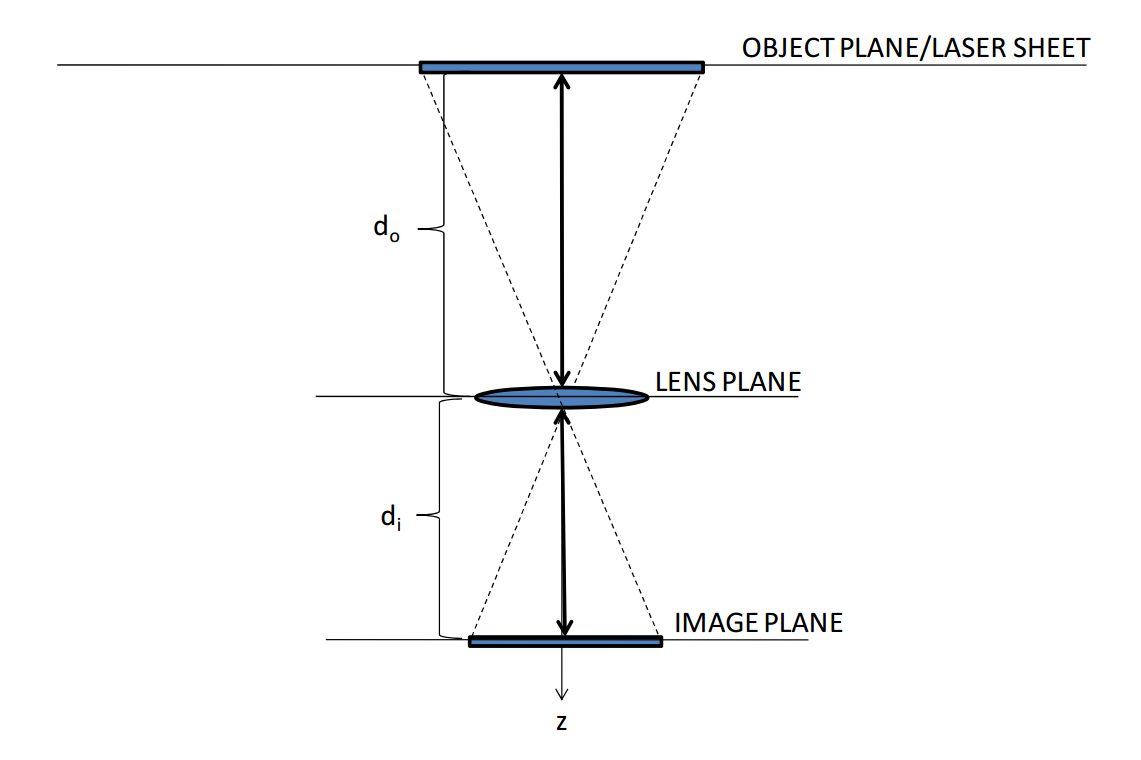
\includegraphics[width=5in]{figs/piv_method/mono_piv_optics}
	\caption{Single camera PIV system for mapping two dimensional velocity 
	vectors}
	\label{fig:mono_piv}
\end{figure} 


\begin{figure}[H]
	\centering
	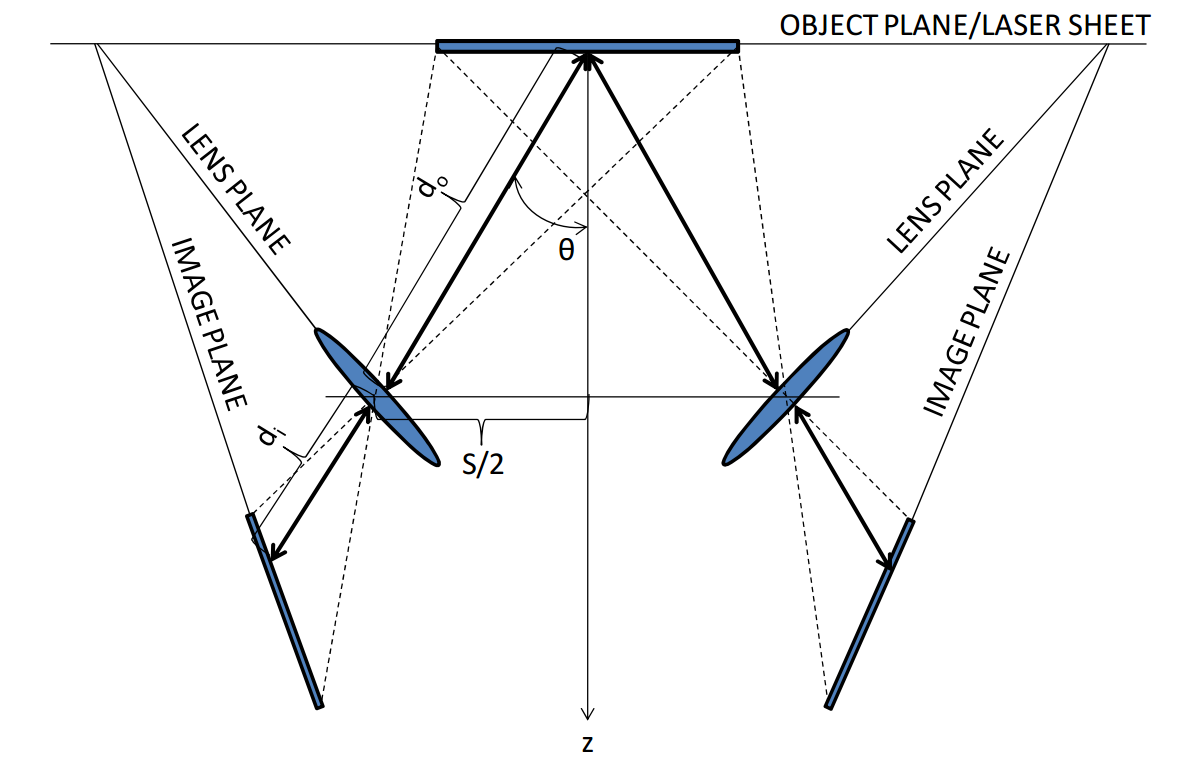
\includegraphics[width=5in]{figs/piv_method/stereo_piv_optics}
	\caption{Stereo camera PIV system for mapping three dimensional velocity 
		vectors}
	\label{fig:stereo_piv}
\end{figure} 


A significant disadvantage is that the sampling rate is restricted by the 
shutter
speed on the cameras, and this shutter speed can easily be slower than the
time scales at which turbulent phenomena may occur. As technology improves,
this disadvantage is slowly vanishing, as cameras with sampling rates on the
order of 20kHz are becoming available, though at extremely high cost. An
additional disadvantage which also erodes with improved computing power is the
relatively high computational intensity of processing large volumes of raw
image data into fully resolved vector fields, especially at a high sampling
rate.


The present study uses a stereo PIV system which resolves three dimensional 
vectors gridded to a two dimensional cross section of flow. The cameras used 
are  are capable of taking two images a few microseconds apart, 
but cannot fully open and close the shutter that quickly. Deriving velocity 
vectors requires two images just a few microseconds apart, but pairs of images 
can be taken at greater time intervals. The PIV method used in this study 
relies upon a frame straddling technique, that times laser pulses at the edges 
of the camera exposures in order to meet this requirement. This results in two 
cameras, which simultaneously take a pair of images, and 25-50 microseconds 
later take a second pair of snapshots for a total of four images, Ra, Rb, La, 
and Lb (flag, math notation). This can be repeated once every second, resulting 
in a true sampling frequency of 1Hz.

\subsection{Mathematical Basis}

The mathematics behind derivation of velocity vector fields from stereo image 
pairs is based upon coordinate transformations from pixel coordinates to real 
coordinates with the following equations 
\ref{eq:piv_to_real1} to \ref{eq:piv_to_real4}.

\begin{equation}
	x_L= X\frac{dx_L}{dX} + Y\frac{dx_L}{dY} + Z\frac{dx_L}{dZ}
	\label{eq:piv_to_real1}
\end{equation}

\begin{equation}
	x_R= X\frac{dx_R}{dX} + Y\frac{dx_R}{dY} + Z\frac{dx_R}{dZ}
	\label{eq:piv_to_real2}
\end{equation}

\begin{equation}
	y_L= X\frac{dy_L}{dX} + Y\frac{dy_L}{dY} + Z\frac{dy_L}{dZ}
	\label{eq:piv_to_real3}
\end{equation}

\begin{equation}
	y_R= X\frac{dy_R}{dX} + Y\frac{dy_R}{dY} + Z\frac{dy_R}{dZ}
	\label{eq:piv_to_real4}
\end{equation}

where $x_L$, $x_R$, $y_L$ and $y_R$ are the pixel displacements in the x 
direction on the left and right cameras, and the y direction on the left and 
right cameras respectively. Symbols $X$, $Y$, and $Z$ are real spatial particle 
displacements in the interrogation plane. The set of twelve derivatives are 
pixel displacement sensitivity coefficients, which are determined by a 
calibration process which involves taking pictures of a matrix of bright dots 
with a known distance between each dot. Once all twelve calibration 
coefficients are known, the set of equations is actually over constrained, with 
four equations and only three unknowns, a least squared method will be used to 
map measurements form the image plane to the real plane. In the case of this 
study, INSIGHT software was used to generate this set of calibration 
coefficients.

Pixel displacements are computed by significantly up sampling the images by 
interpolation, dividing each image into many small sectors, and 
comparing an  image $A$ with a image $B$ with a correlation map. The image is 
up sampled to higher resolution to allow sub-pixel displacements to be 
measured, thus preventing accuracy limitations associated with the physical 
dimensions of each pixel. The image is typically divided into grids 16 by 16 
pixels in size, with 50\% overlap with surrounding grids to ensure particles 
which started inside the sector at $t=0$, but begin to exit the sector at 
$t=dt$, are still identifiable.  The correlation map is computed by taking the 
inverse fast Fourier transform (FFT)of the product of the FFT of the first 
image, and the complex conjugate of the FFT of the second image, then adjusting 
for up-sampling by dividing by the original factor as in equation 
\ref{eq:correlation_map}.

\begin{equation}
	C_{map} = FFT^{-1} * [F_A \times conj(F_B) ]
	\label{eq:correlation_map}
\end{equation}

where $C_{map}$ is the correlation map, $F_A$ is the fast Fourier transform of 
image $A$, at time $t=0$ and $F_B$ is the fast Fourier transform of image $B$ 
at time $t=dt$.

Figure \ref{fig:piv_sector_0up} shows a sample of two side by side images taken 
several microseconds, $dt$ apart without any up-sampling. Figure 
\ref{fig:piv_sector_overlay_fft_0up} shows a sample of the same two images 
layered on top of each other to show the apparent horizontal displacement 
between the two images. The two dimensional correlation map shows a clear peak 
down at four pixels in the $X$ direction and zero pixels in the $Y$ direction.


\begin{figure}[H]
	\begin{subfigure}{.5\textwidth}
		\centering
		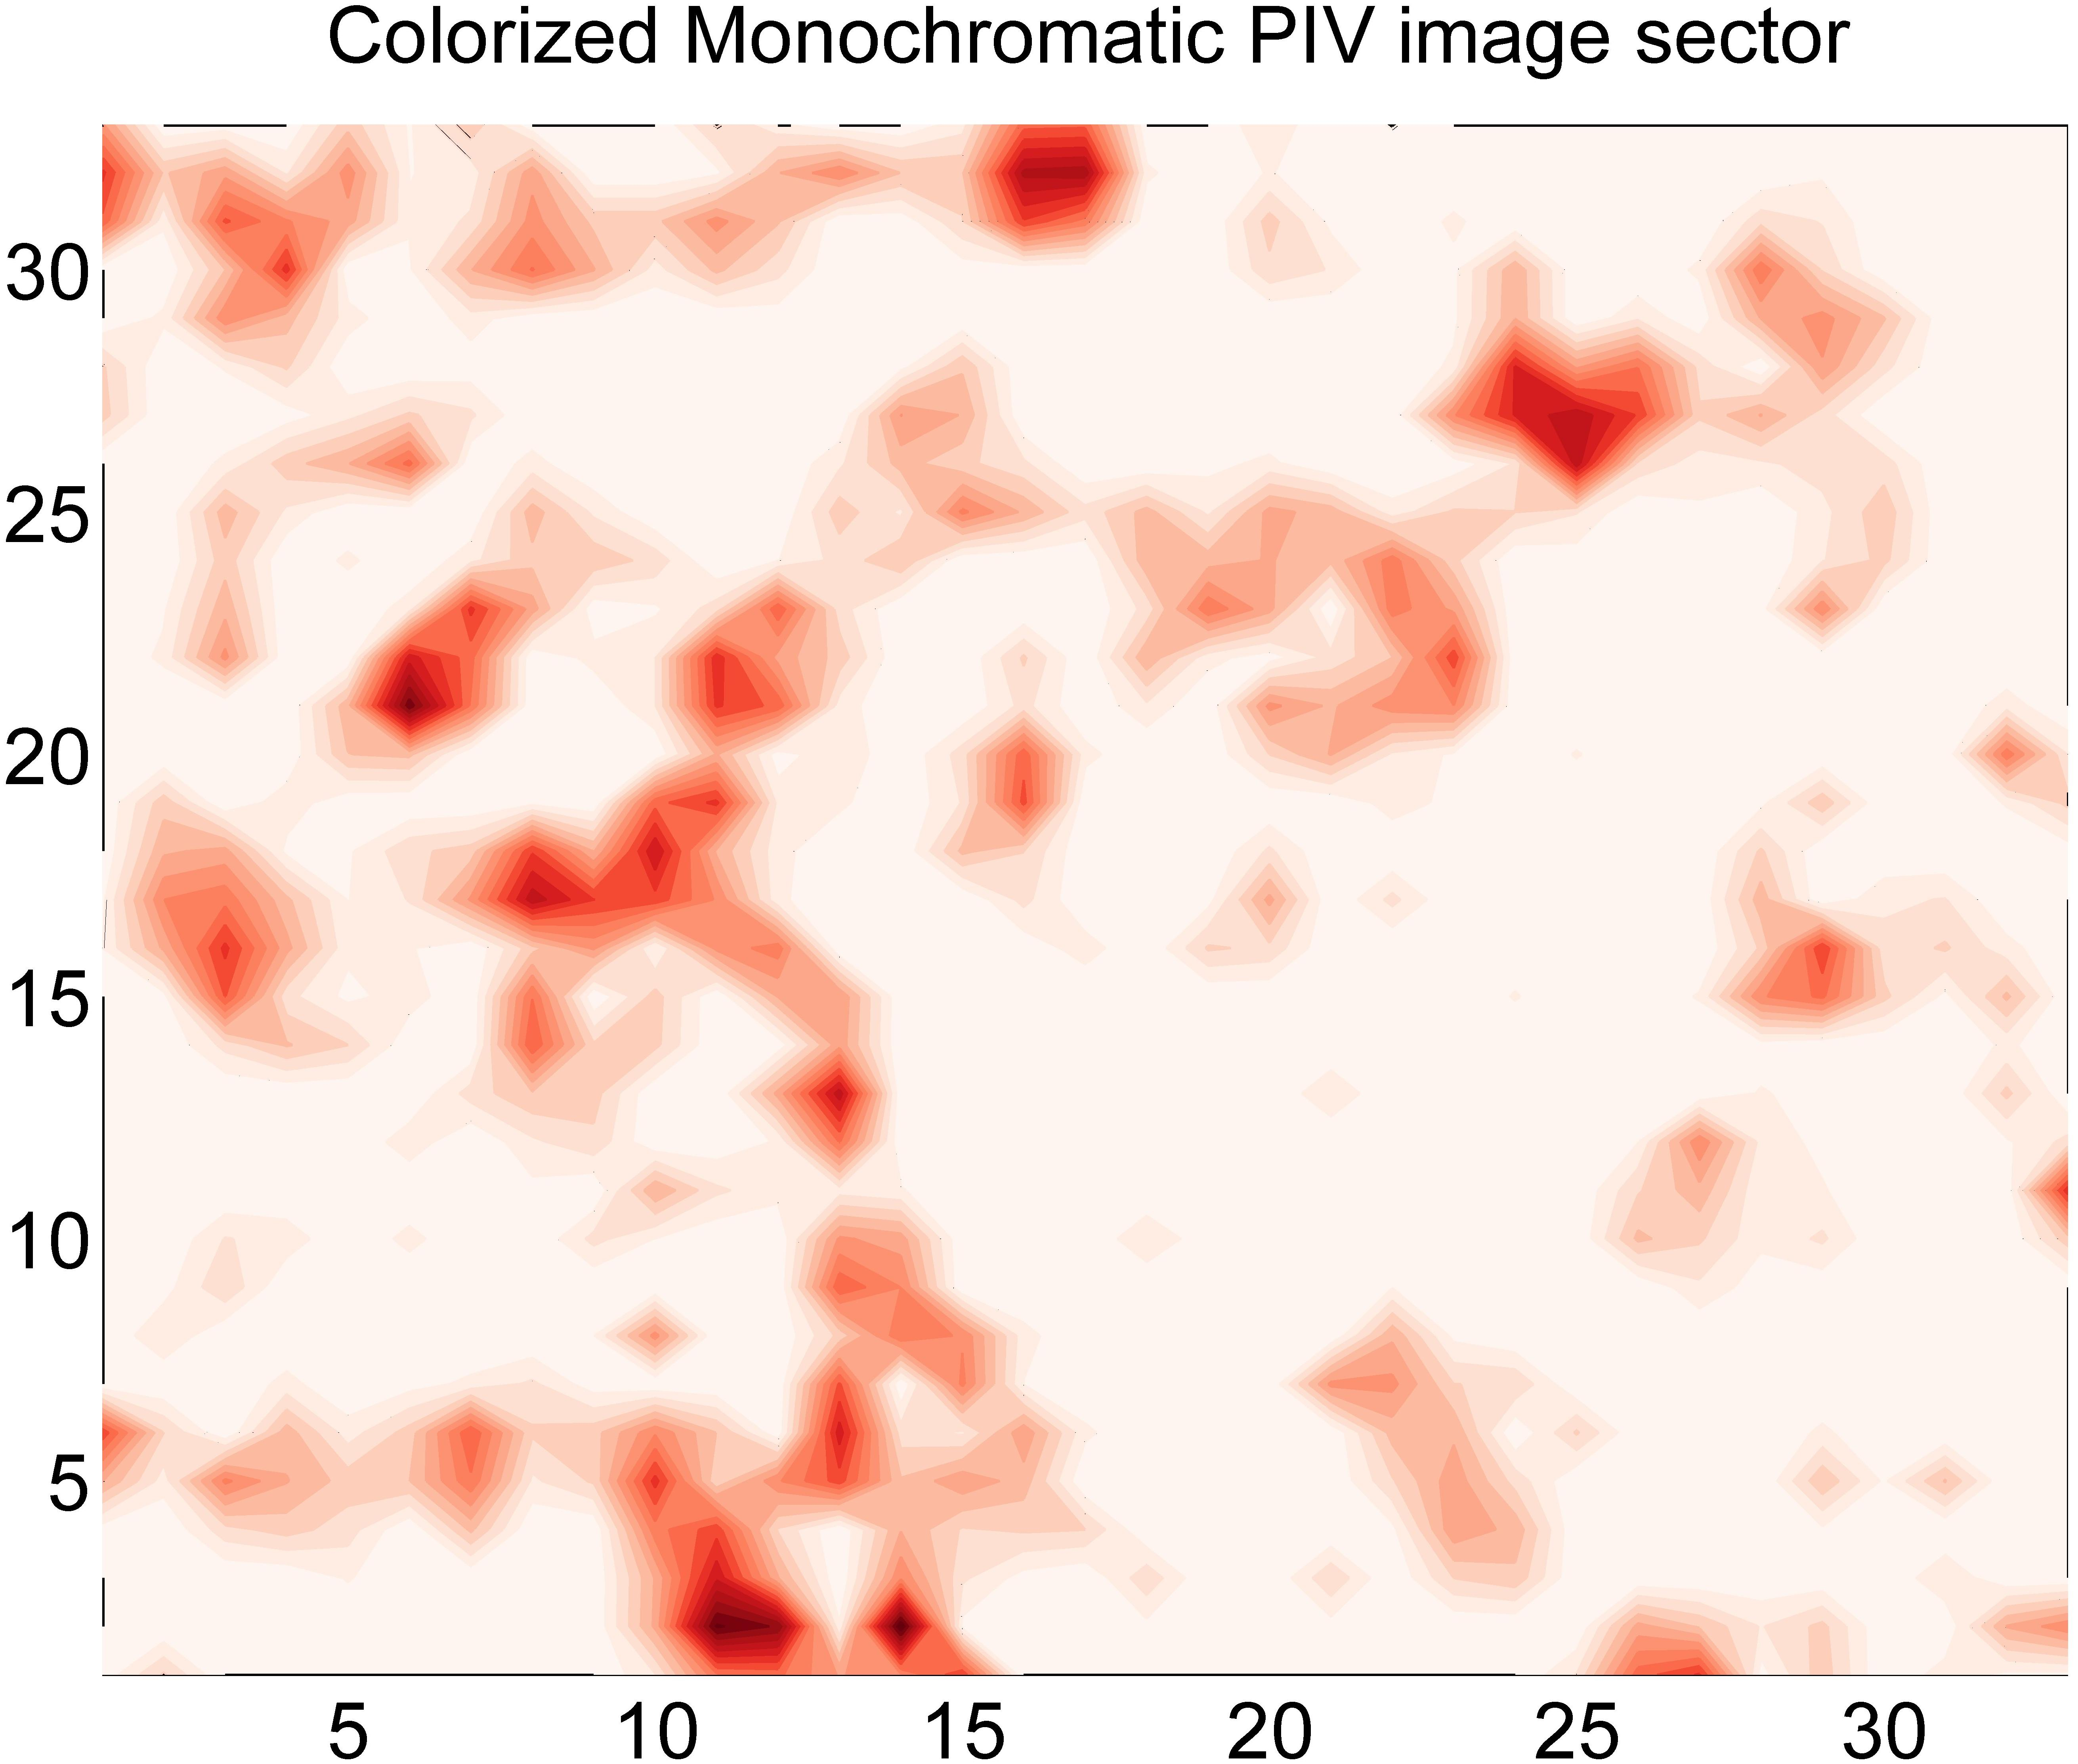
\includegraphics[width=.8\linewidth]{figs/piv_method/pive_figa_order0}
	\end{subfigure} 
	\begin{subfigure}{.5\textwidth}
		\centering
		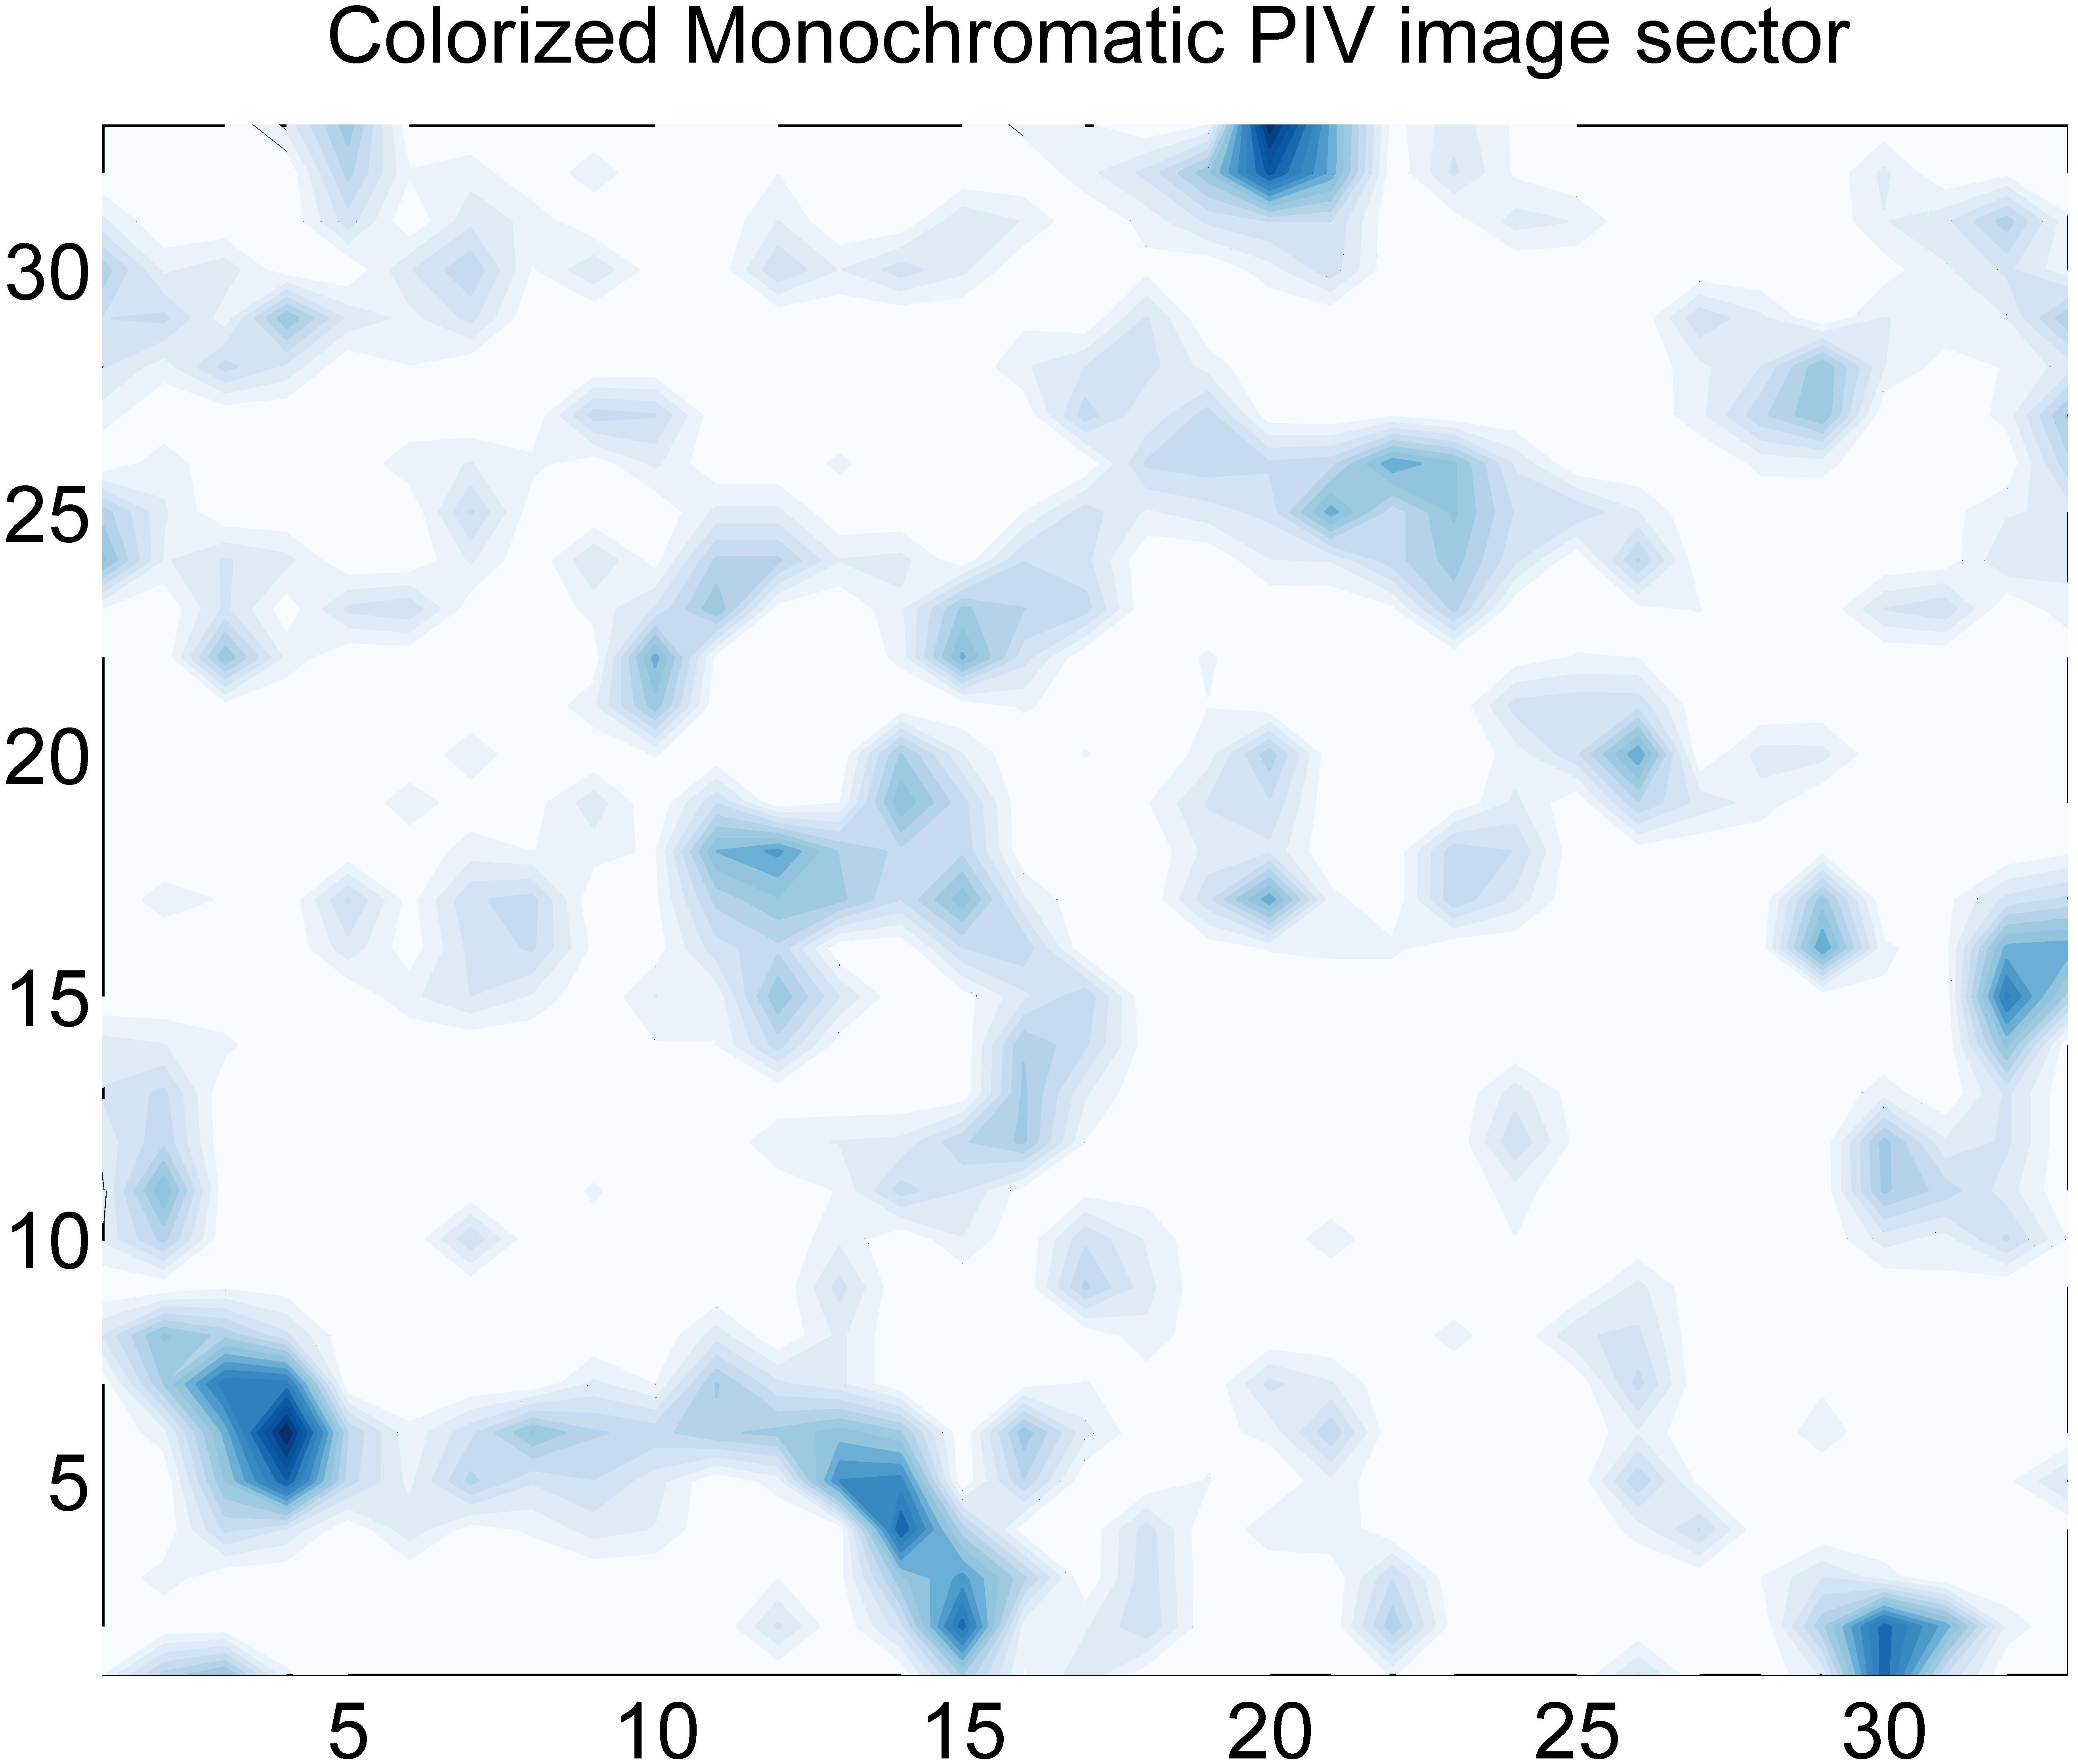
\includegraphics[width=.8\linewidth]{figs/piv_method/pive_figb_order0}
	\end{subfigure}	
	\caption{Colorized 32x32 pixel contour images at $t=0$ (left), and $t=dt$ 
	(right), no up sampling.}
	\label{fig:piv_sector_0up}
\end{figure}


\begin{figure}[H]
	\begin{subfigure}{.5\textwidth}
		\centering
		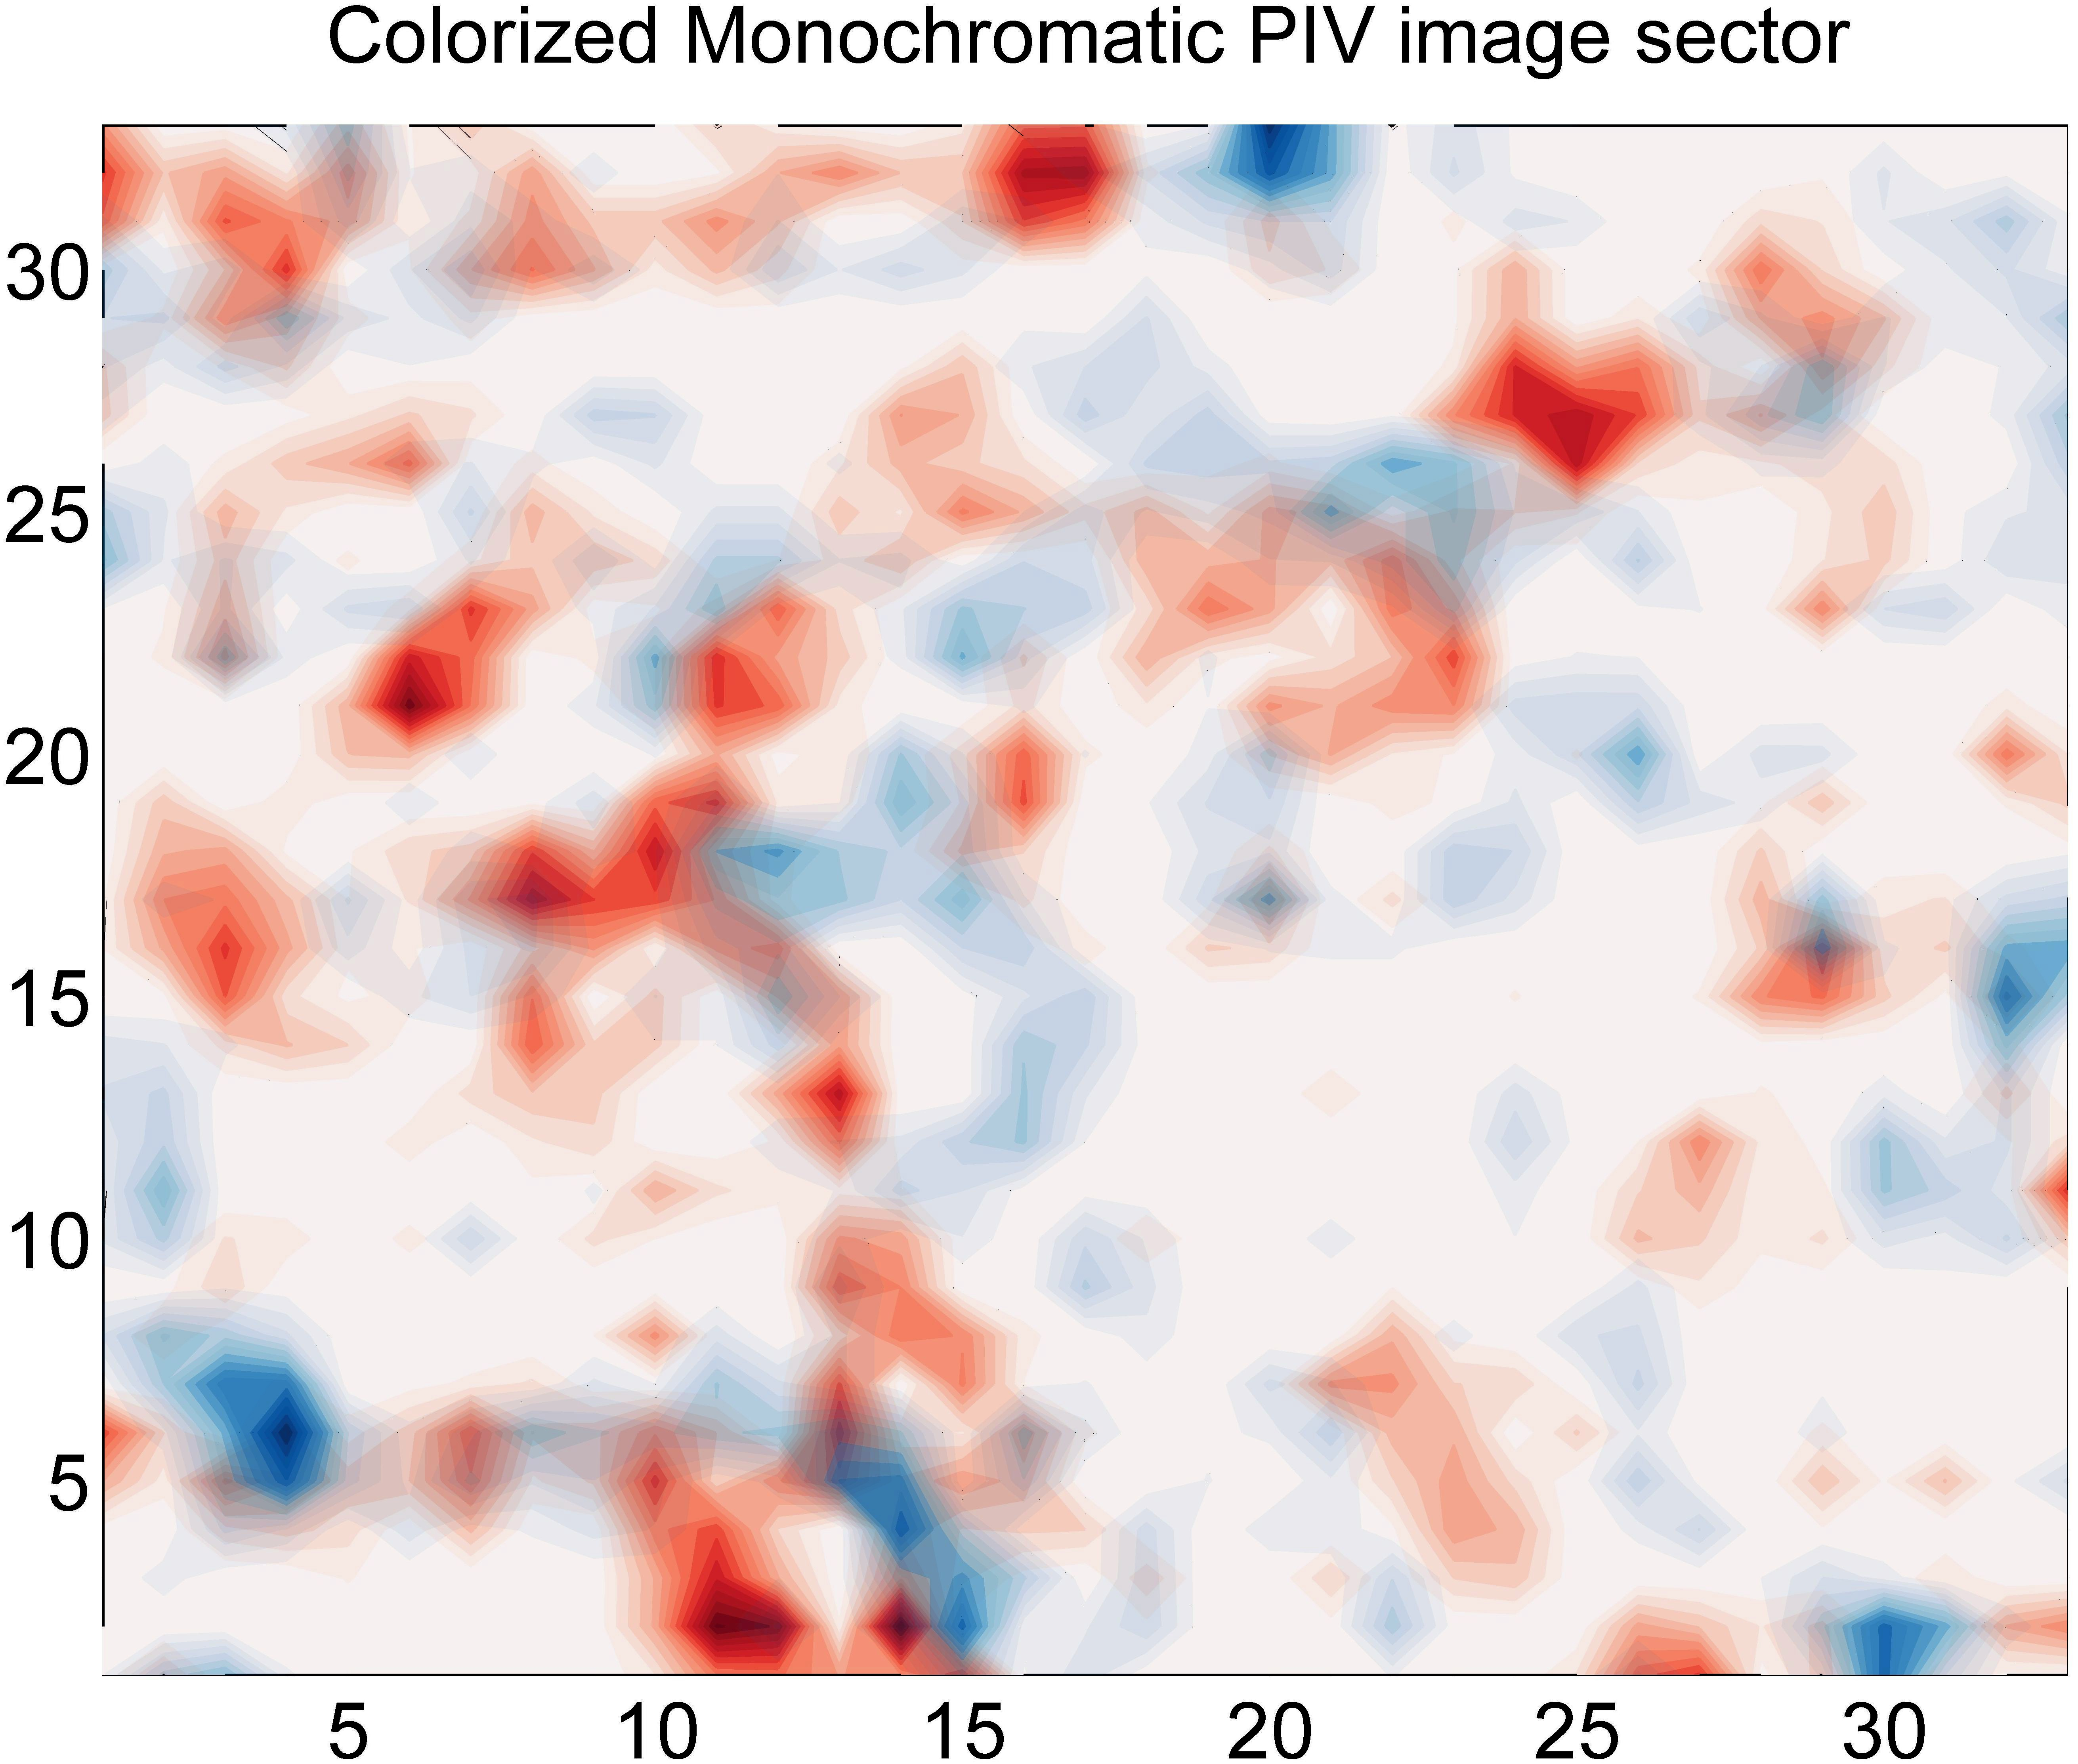
\includegraphics[width=.8\linewidth]{figs/piv_method/pive-fig_order0}
	\end{subfigure} 
	\begin{subfigure}{.5\textwidth}
		\centering
		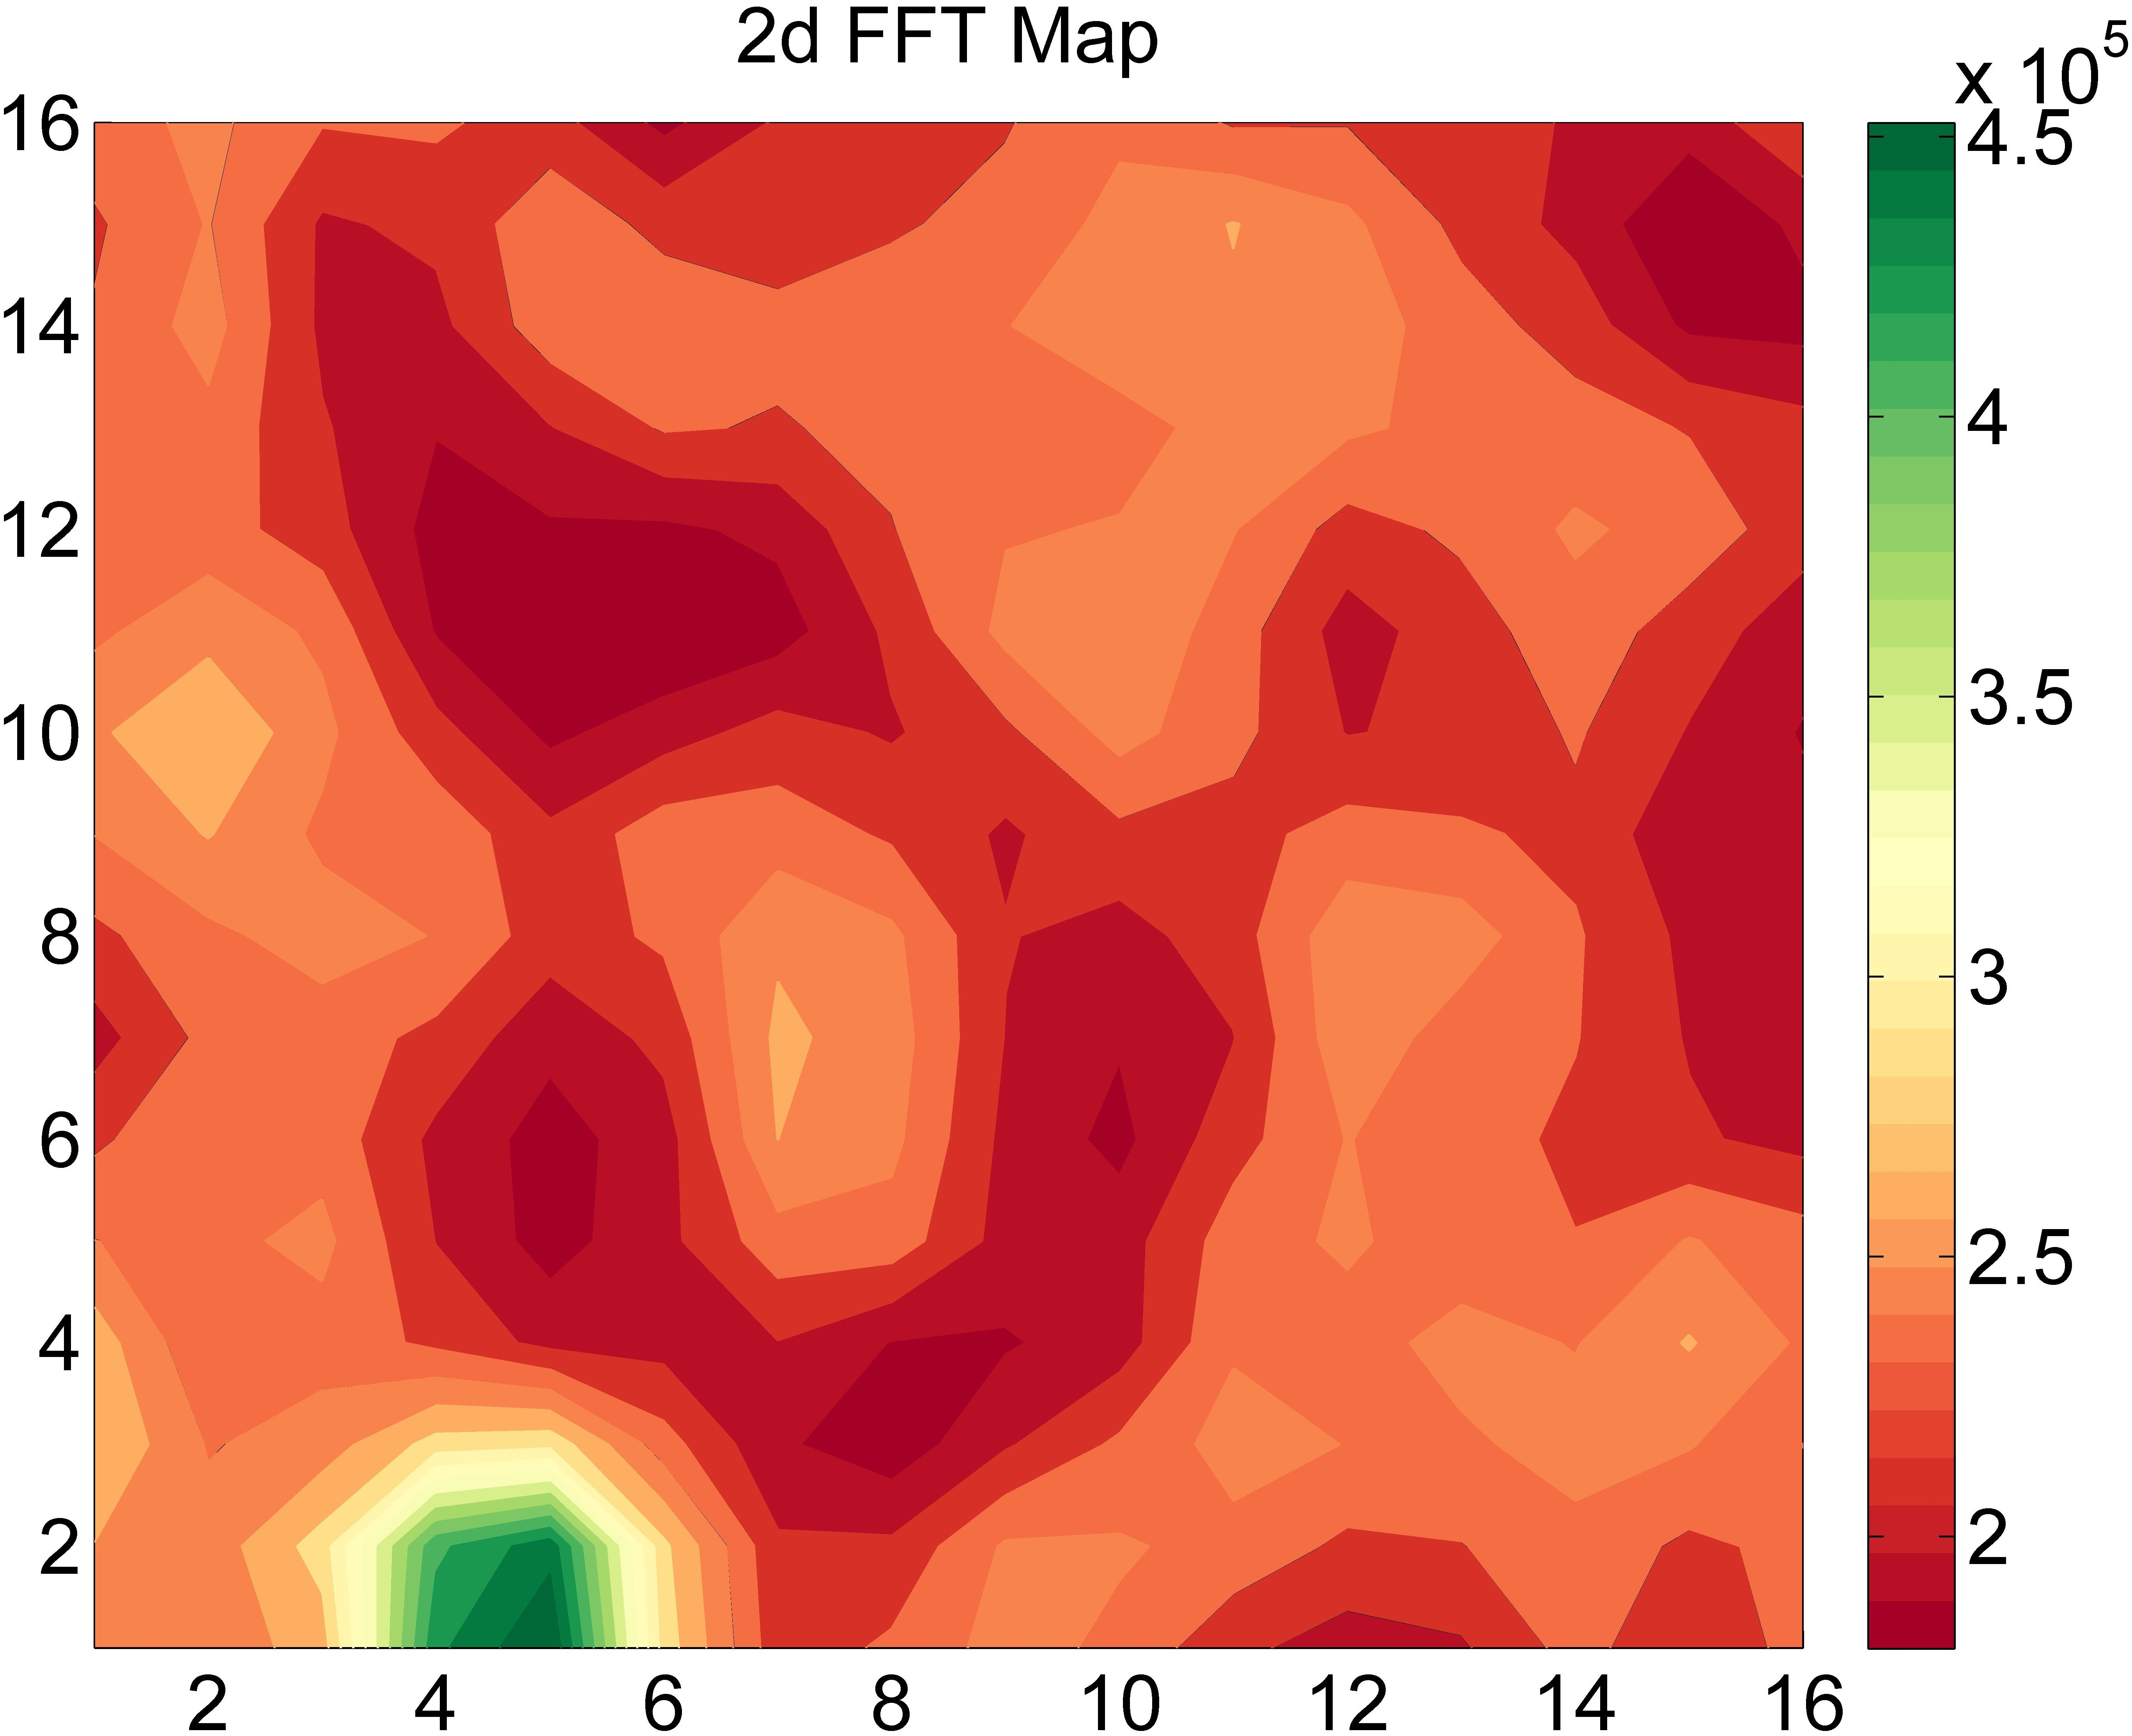
\includegraphics[width=.8\linewidth]{figs/piv_method/pive_fft_order0}
	\end{subfigure}	
	\caption{Overlaid sector snapshots (left) and corresponding correlation 
	map (right), no up sampling.}
	\label{fig:piv_sector_overlay_fft_0up}
\end{figure}


Every up sampling doubles the dimensions of the sector, quadrupling the number 
of pixels and increasing the sub-pixel resolution by a factor of two. The same 
set of figures is repeated for the same image with 6th order bilinear up 
sampling in figures \ref{fig:piv_sector_6up} and
\ref{fig:piv_sector_overlay_fft_6up}. Note that the images are much smoother, 
and the images have been sampled sufficiently to make a very finely spaced grid.
It is important to note that while bilinear up sampling is used for this
example, any other two dimensional method such as cubic may be used.

\begin{figure}[H]
	\begin{subfigure}{.5\textwidth}
		\centering
		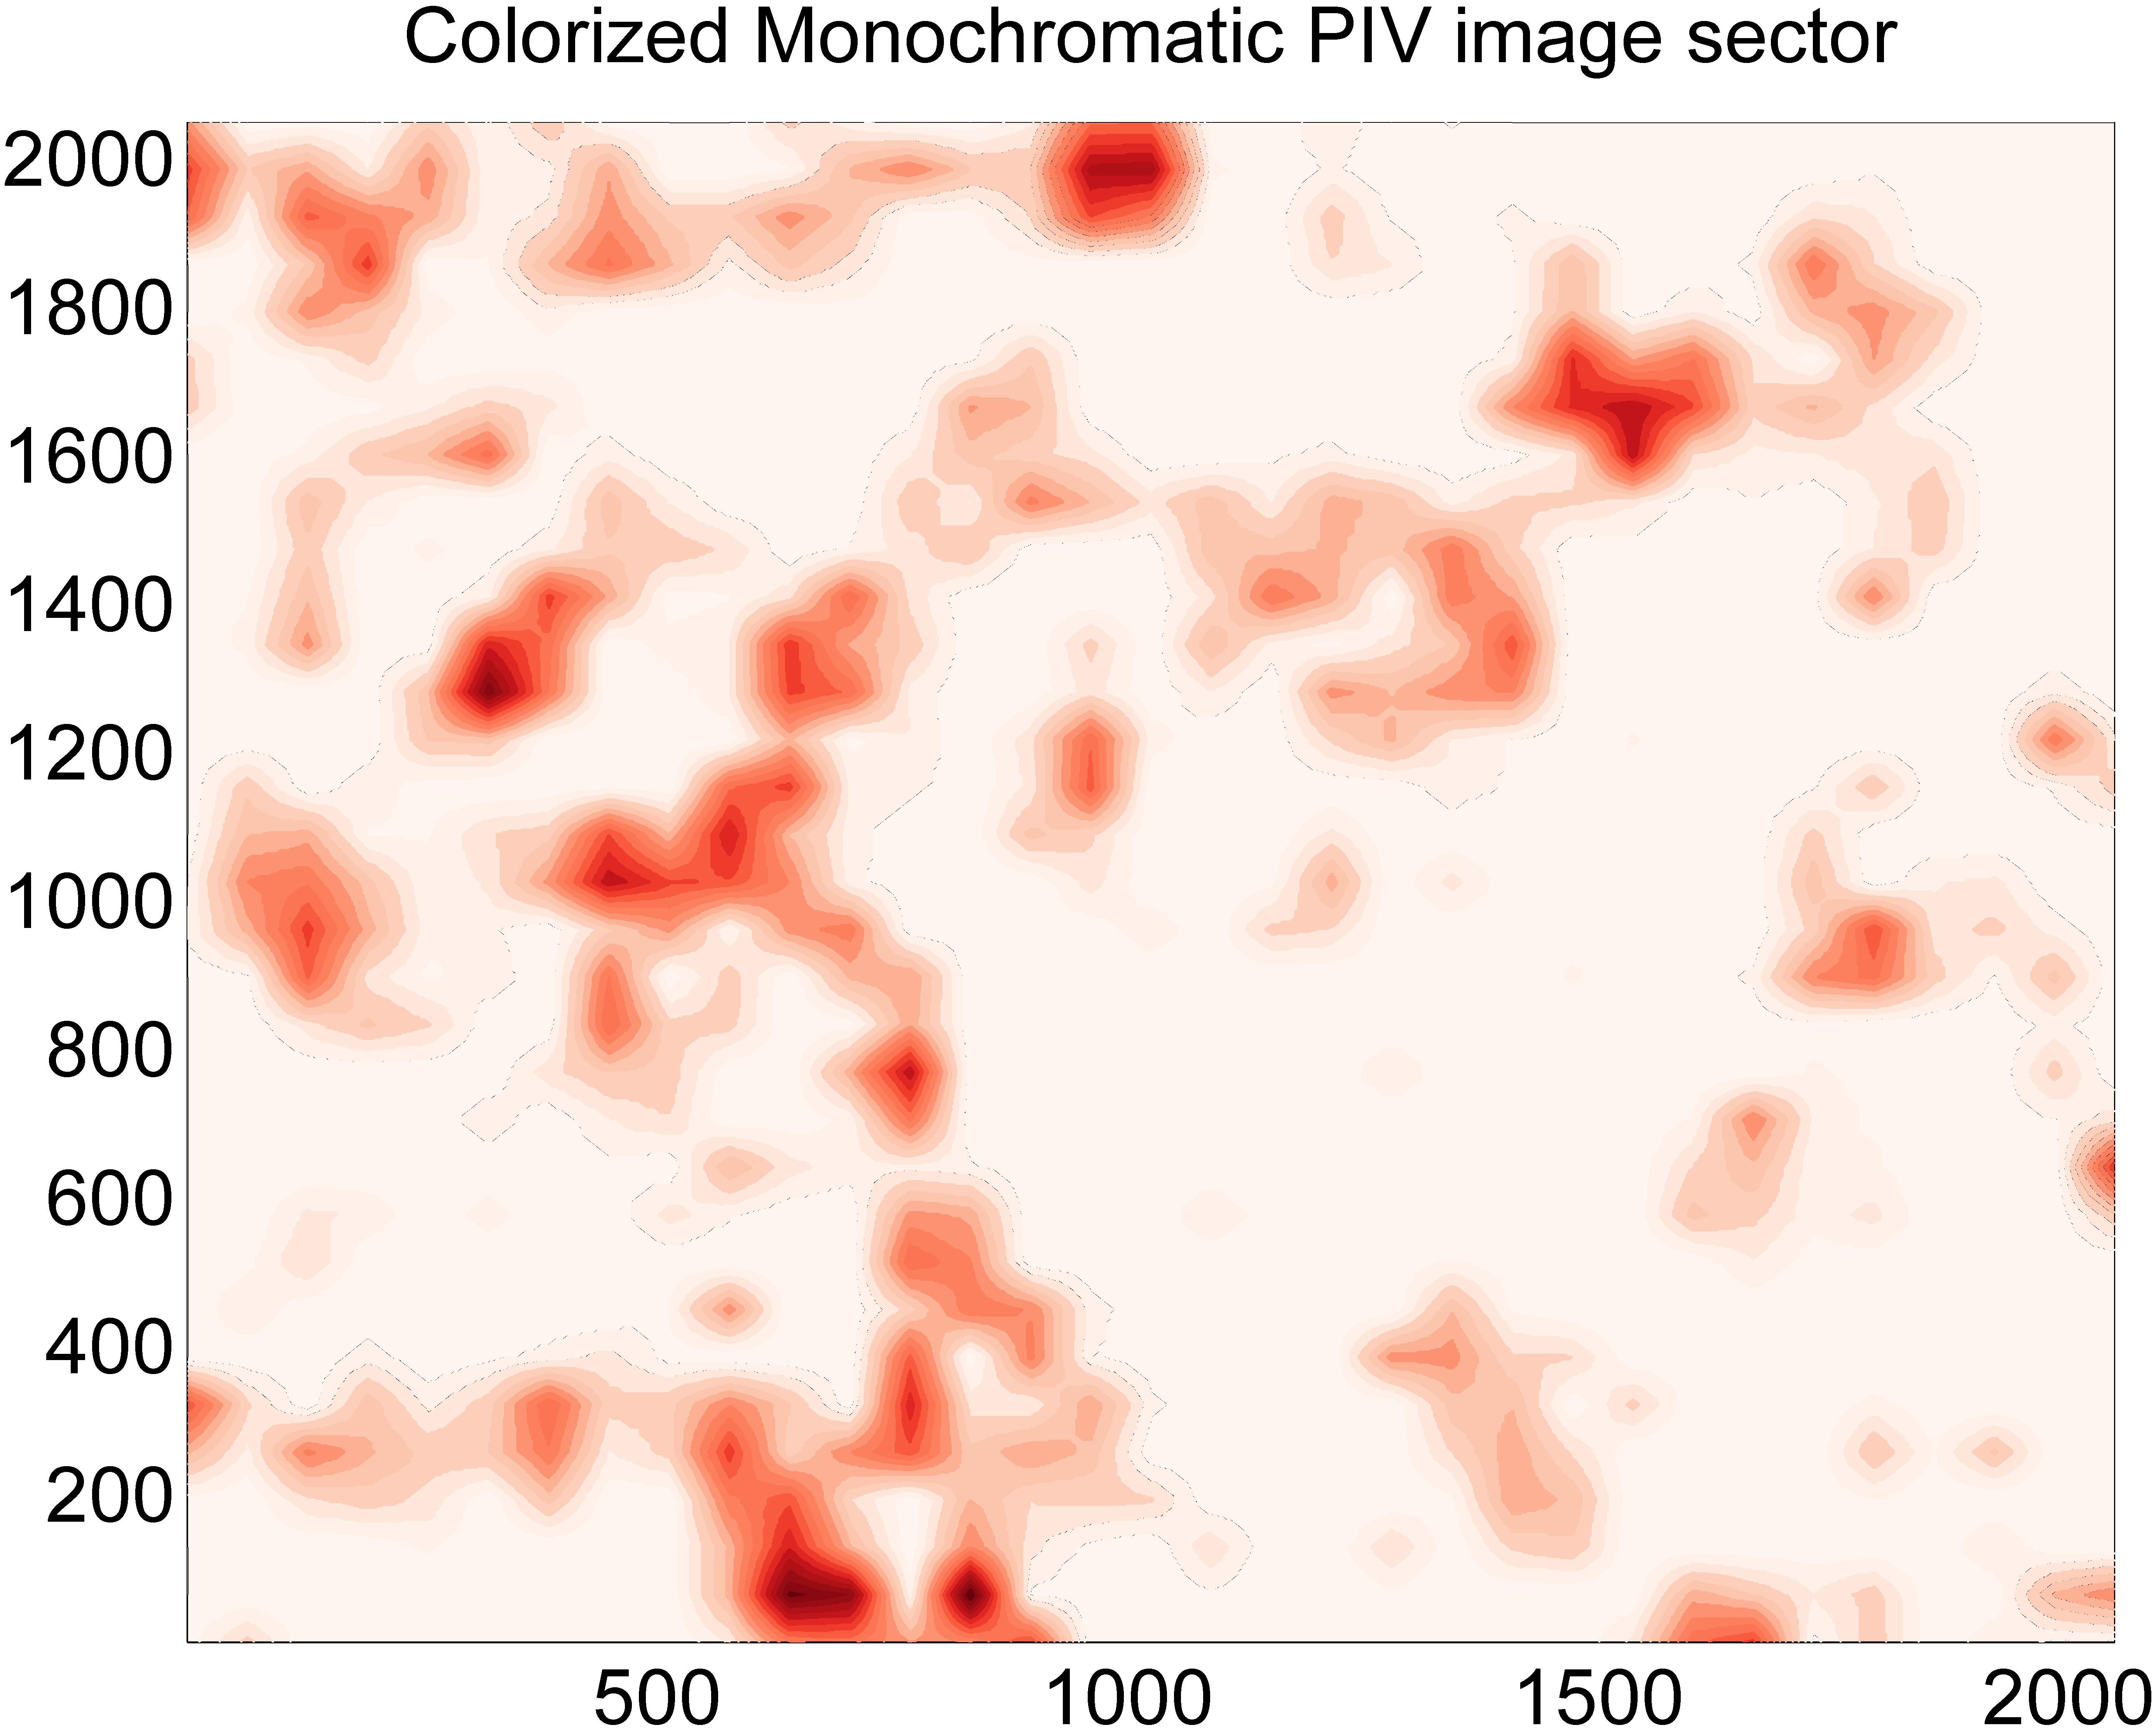
\includegraphics[width=.8\linewidth]{figs/piv_method/pive_figa_order6}
	\end{subfigure} 
	\begin{subfigure}{.5\textwidth}
		\centering
		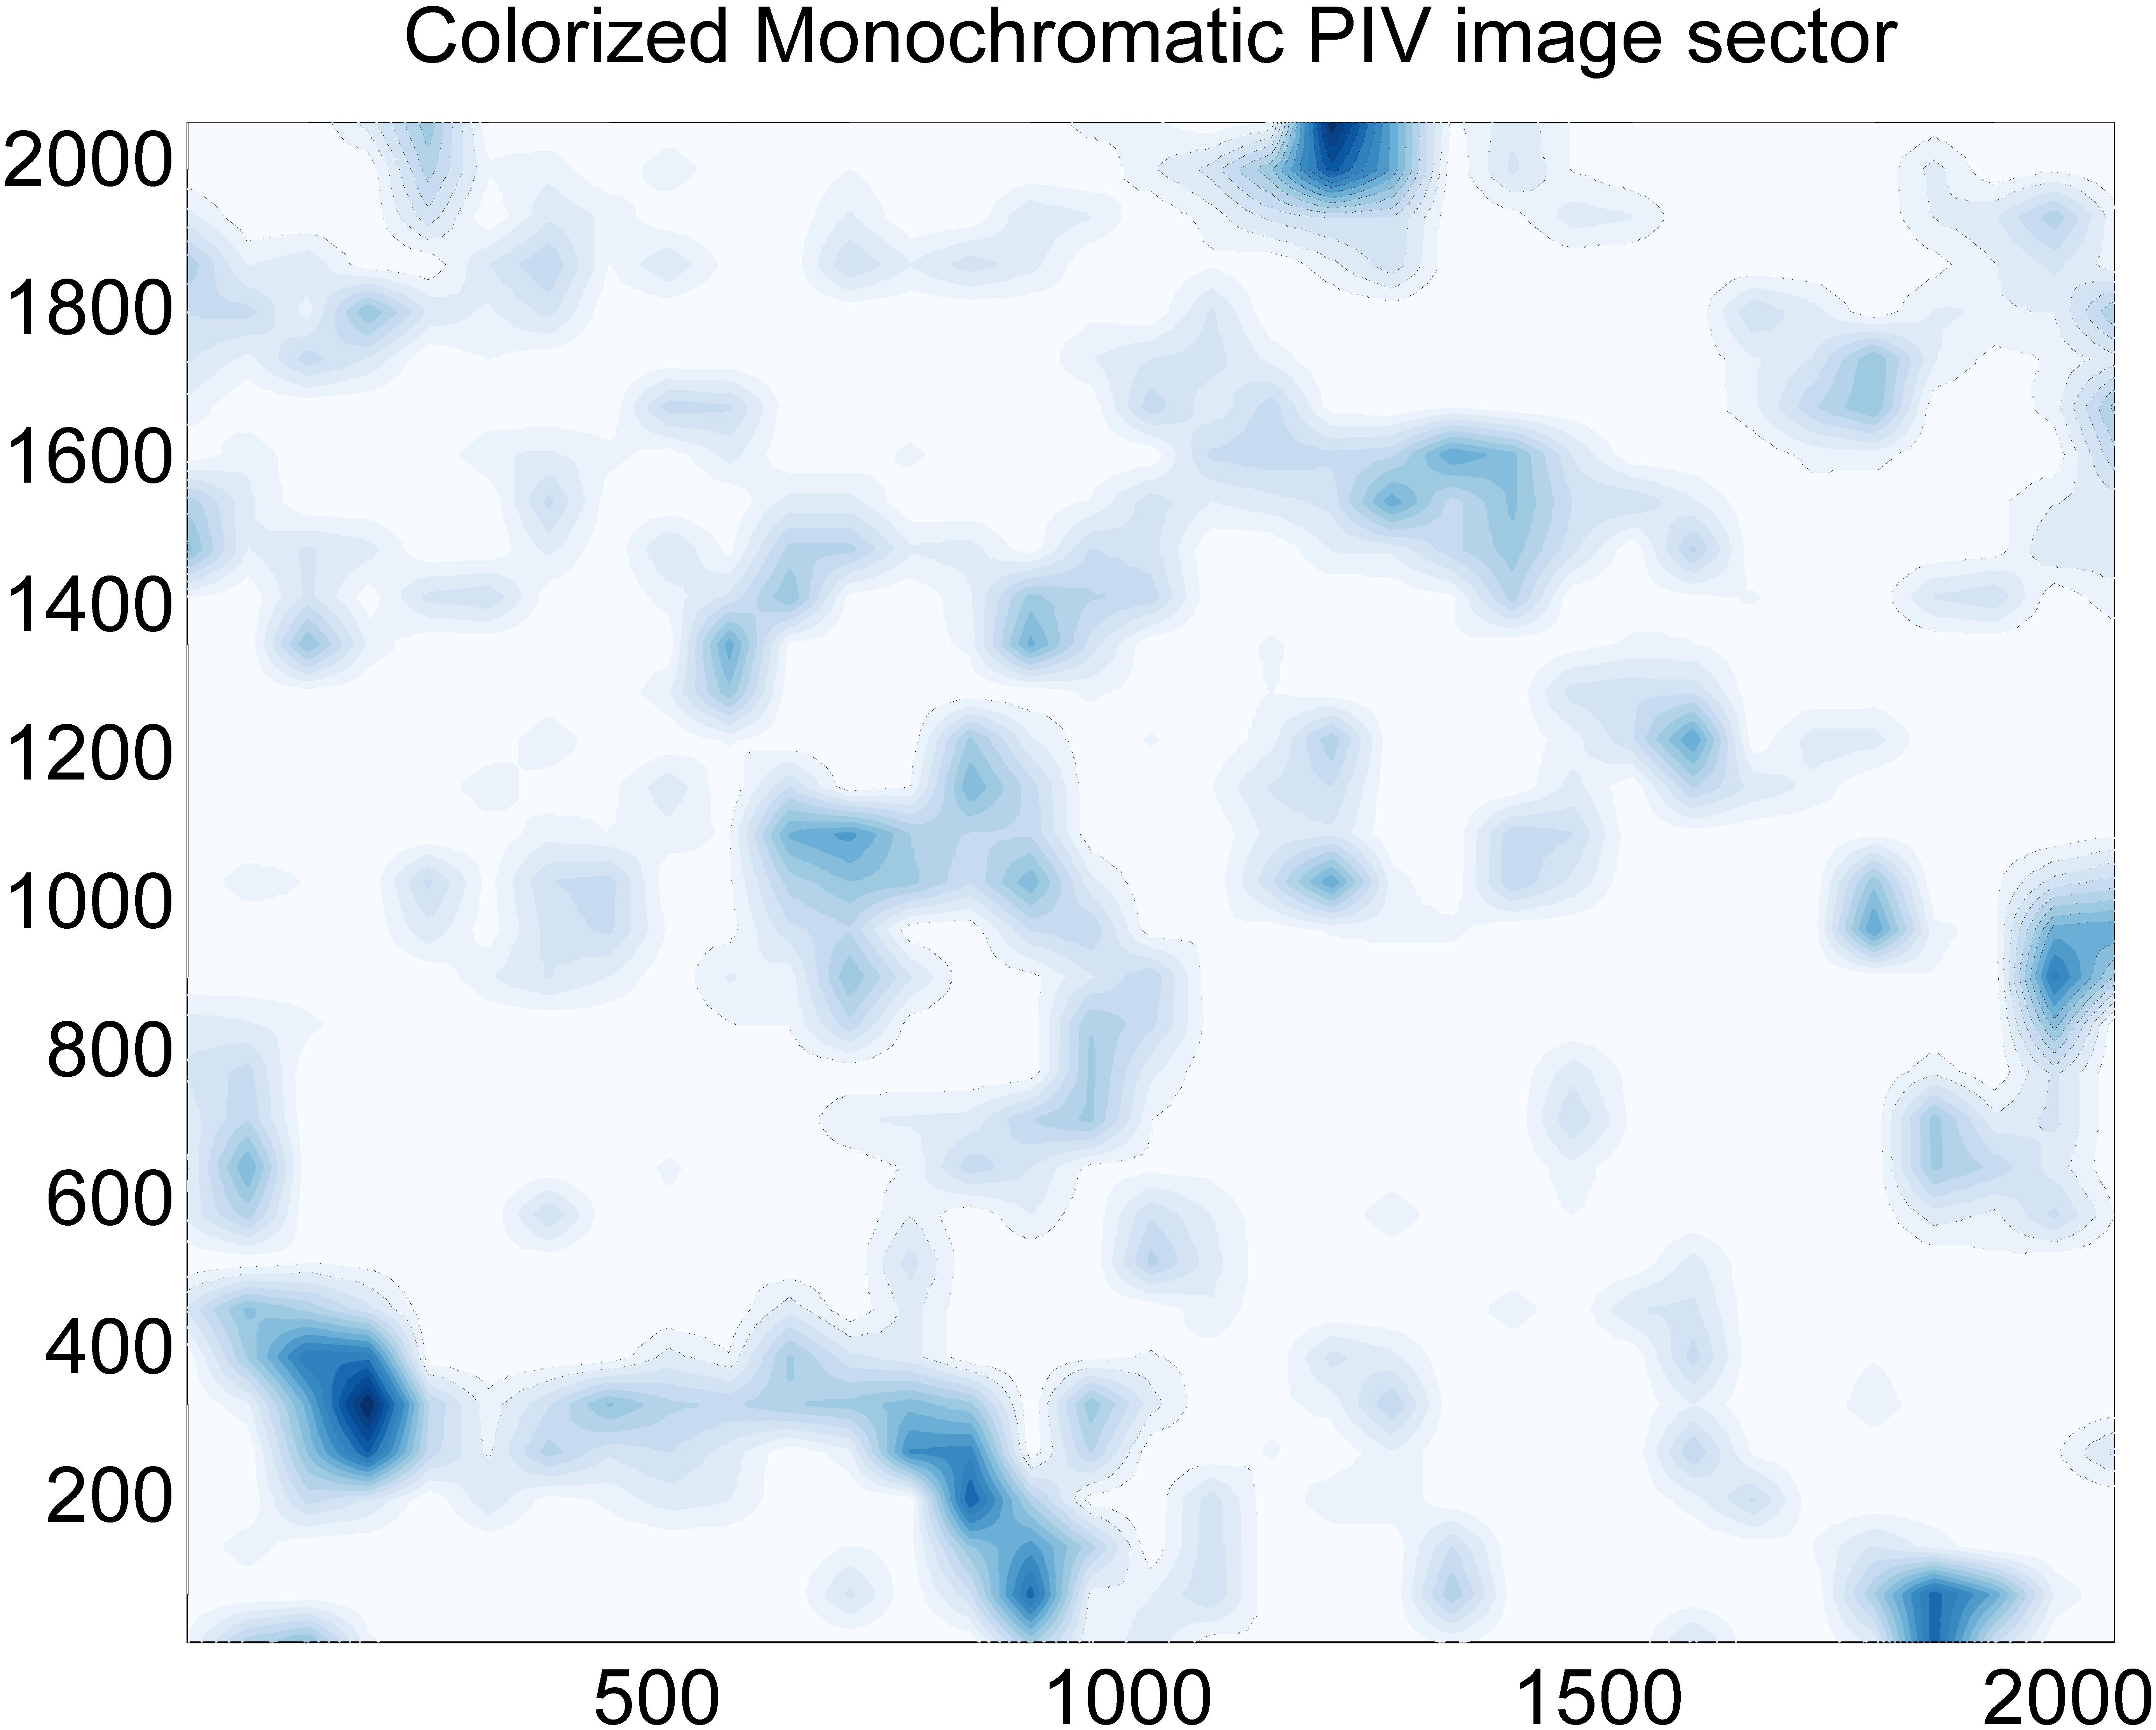
\includegraphics[width=.8\linewidth]{figs/piv_method/pive_figb_order6}
	\end{subfigure}	
	\caption{Colorized 32x32 pixel contour images at $t=0$ (left), and $t=dt$ 
		(right), 6th order up sampling.}
	\label{fig:piv_sector_6up}
\end{figure}


\begin{figure}[H]
	\begin{subfigure}{.5\textwidth}
		\centering
		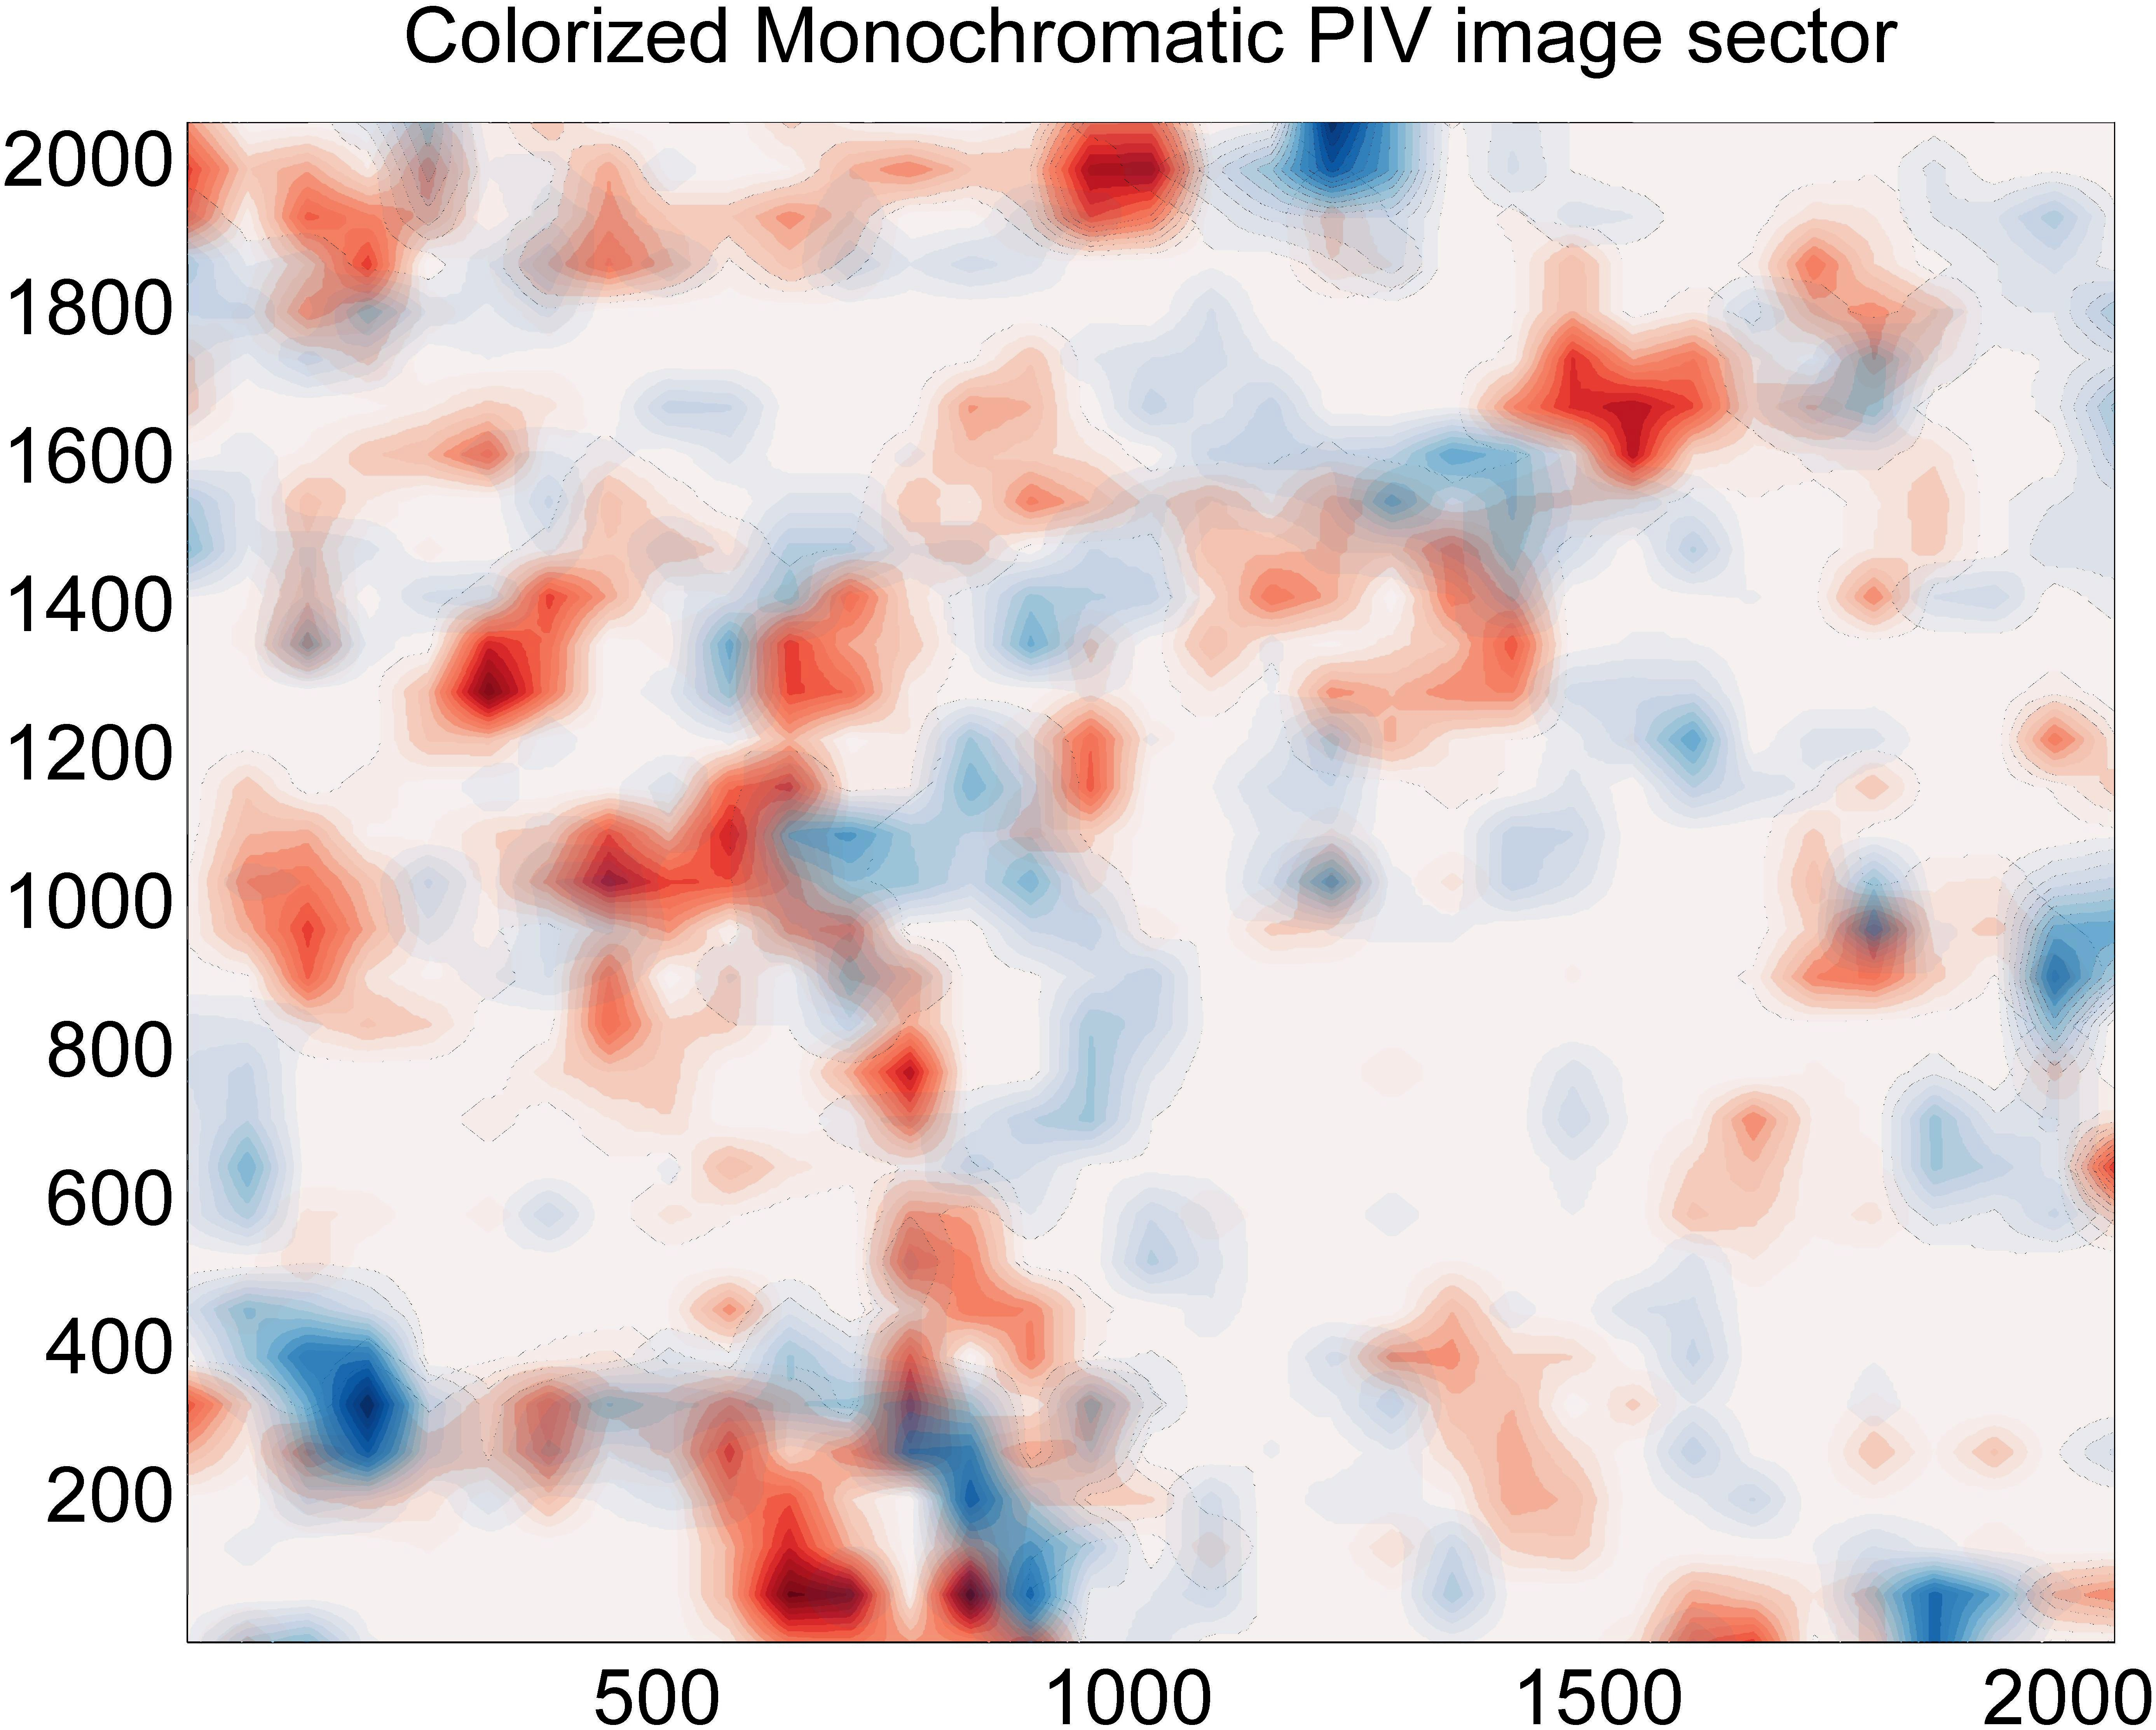
\includegraphics[width=.8\linewidth]{figs/piv_method/pive-fig_order6}
	\end{subfigure} 
	\begin{subfigure}{.5\textwidth}
		\centering
		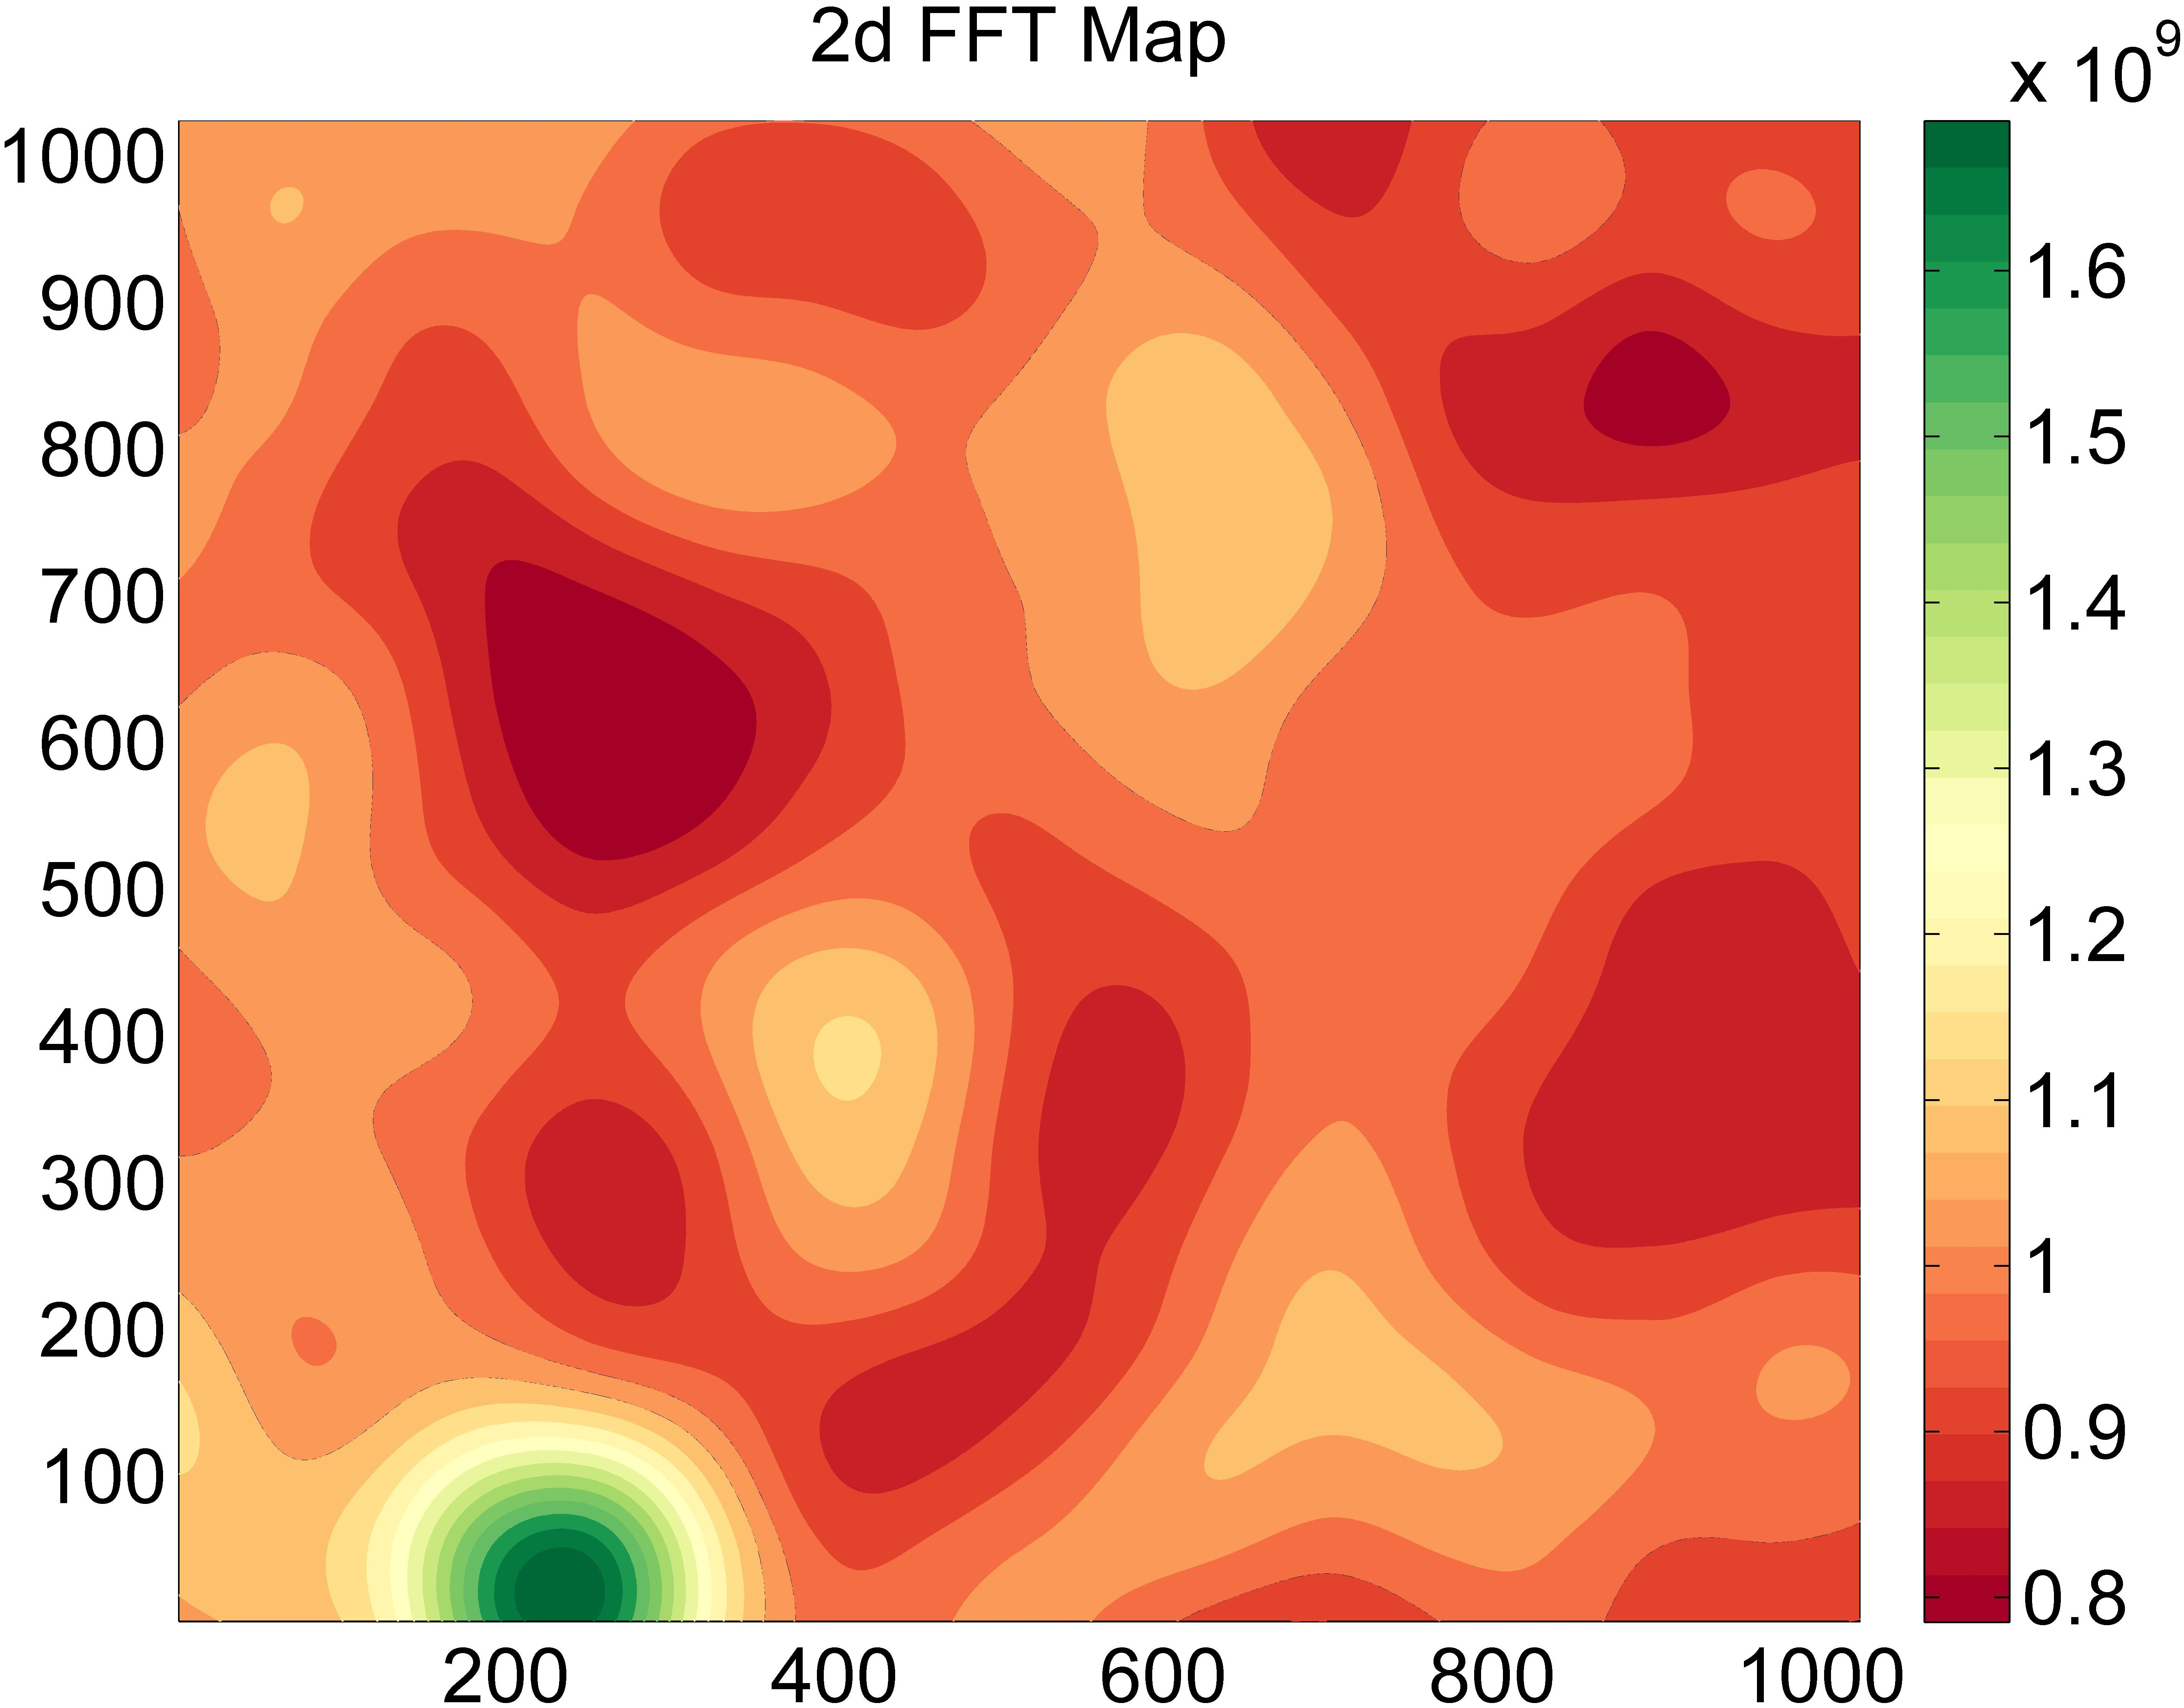
\includegraphics[width=.8\linewidth]{figs/piv_method/pive_fft_order6}
	\end{subfigure}	
	\caption{Overlaid sector snapshots (left) and corresponding correlation 
		map (right), 6th order up sampling.}
	\label{fig:piv_sector_overlay_fft_6up}
\end{figure}

As the sampling method creates a finer mesh, the sub-pixel resolution 
increases. Table \ref{table:piv_upsampling_displacement} shows how the 
displacement error may vary with sampling order.

\begin{table}[H]
\begin{center}
\begin{tabular}{|ccc|}
	\hline
	Order & $x_{disp}$ & $y_{disp}$\\
	\hline
	0 & 4 & 0\\
	1 & 3.5 & 0.5\\
	2 & 3.75 & 0.25\\
	3 & 3.625 & 0.25\\
	4 & 3.625 & 0.3125\\
	5 & 3.625 & 0.3125\\
	6 & 3.6406 & 0.2969\\
	7 & 3.6406 & 0.2969\\
	\hline
\end{tabular}
\caption{Pixel displacements by up sampling order.}
\label{table:piv_upsampling_displacement}
\end{center}
\end{table}


While the above analysis demonstrates the mathematical motivation behind up 
sampling images before performing a Fourier transform for measuring particle 
displacement, it does not adequately describe the total uncertainty in 
measurements made with particle image velocimetry. The uncertainty associated 
with measurements made with PIV are dependent upon the geometry of the specific 
optical setup used to take the data.


\subsection{Seeding the Flow}

Appropriate particle seeding density and time between straddled frames is the
subject of continued study, and is difficult to predict before hand. 
Completeness of a two dimensional vector field is highly dependent upon 
uniform
optimal particle density conditions which are difficult to obtain, and maintain
over an extended test. For stereo PIV, incomplete data in either of the two 
dimensional vector 
sets from either camera at a given spatial location will result in an 
indeterminate vector displacement in the three dimensional vector data. To 
elevate the likelihood that a displacement vector at a given location can be 
properly determined, an additional data refining technique outlined in Hart 
(flag, reference) was employed. The Hart method compares correlation maps 
between two adjacent sectors for consistency. in instances where two adjacent 
regions lack a well-defined peak, the Hart method functions to magnify shared 
peaks and reveal a solution that might otherwise have been missed. In instances 
where sub optimal seeding conditions were present and a correlation map 
produces a false peak, the Hart method functions to rule the peak out as an 
anomaly if the adjacent sectors do not also indicate a high correlation at that 
location. The way in which in which the Hart method reduces the number of 
erroneous vectors present in a data set is difficult to quantify on a case by 
case basis, but any impact on overall uncertainty of the PIV measurements is 
expected to have a reducing effect. 